\subsection{Output Operating Range}

Since there is no direct translation between the output signal from the board and the speed of the motor and the ESC allows more current than the motor can recognise, it is necessary to find the operating range for the board output that has the most noticeable effect on the RPM of the motor. Through trial and error and by measuring the RPM using SHIMPO DT-205 digital tachometer. The lowest operating point was found to be 762$\mu s$, at which the motor finally begins to spin. The highest point was defined at 1200$\mu s$. Higher values were found to have very small effect on the RPM.
Therefore, despite the ESC recognising the values between 700 and 2000$\mu s$, the most noticeable effect will be between 762 and 1200$\mu s$ and will be primarily used in the project.

\subsection{APM Frequency}
Due to lack of proper documentation, it was necessary to do measure the frequency of the signals sent out by the flight controller. To do so, an oscilloscope was connected to one of the output pins of the board. Then, using the servo library, a signal was sent out. The interval between signals was found to be 20$ms$, therefore, the frequency of the board is 50$Hz$, as seen in figure \ref{oscillo1}.
\begin{figure}[H]
  \centering
    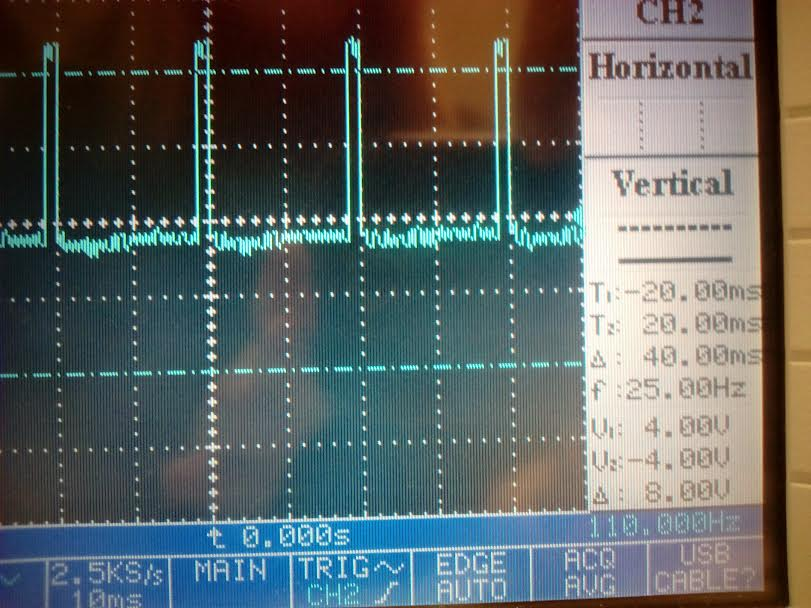
\includegraphics[width=0.5\textwidth]{images/oscillo1.jpg}
	\caption{Oscilloscope measuring APM's frequency.}
	\label{oscillo1}
\end{figure}

The second experiment on the board was then made to determine how the flight controller handles the output signals during those 20$ms$. First two outputs of the APM were connected to the oscilloscope, both utilizing the Servo library to send signals of length of 2000$\mu s$. Results can be seen in figure \ref{oscillo2}.
\begin{figure}[H]
  \centering
    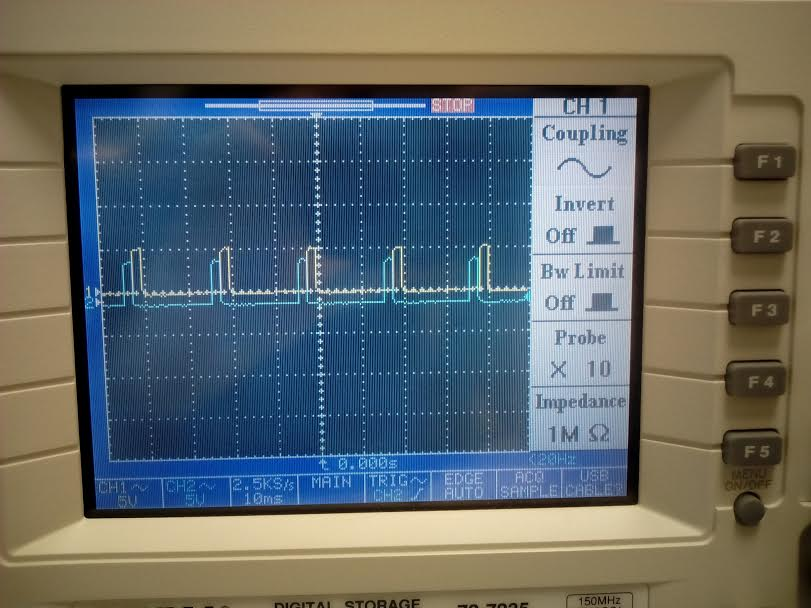
\includegraphics[width=0.5\textwidth]{images/oscillo2.jpg}
	\caption{Readings of the two output signals.}
	\label{oscillo2}
\end{figure}

Then, for further testing purposes, both outputs were given different values in two scenarios, as seen in figure \ref{oscillo3}.

\begin{figure}[H]
  \centering
    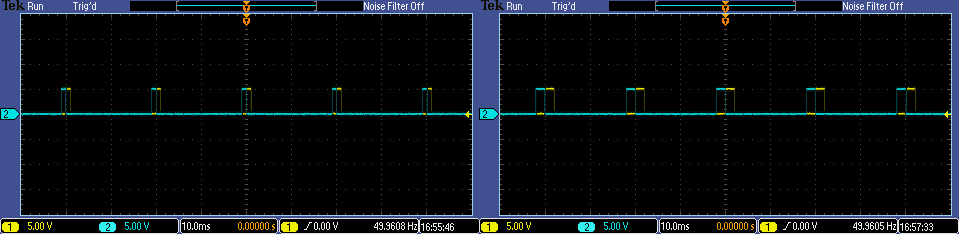
\includegraphics[width=0.5\textwidth]{images/oscillo3.png}
	\caption{Left - signals running at 2000$\mu s$; Right - 700$\mu s$.}
	\label{oscillo3}
\end{figure}

From this, two conclusions can be made:
\begin{enumerate}
\item If the first signal is shorter than the second one, the second signal will still follow right after the first signal ends. In other words, the APM leaves no gaps between the outputs.
\item Since the board runs at the frequency of 50$Hz$ and has a period of 20$ms$, this leaves $\frac{20}{8} = 2.5ms$ maximum length for each output signal. The servo library is hard-capped at 2.4$ms$ and thus is well within the limits of the board.
\end{enumerate}